\documentclass{report}

% PACKAGES
\usepackage[margin=1.00in]{geometry}
\usepackage[pdftex]{graphicx}
\usepackage[table,xcdraw]{xcolor}
\usepackage{indentfirst}
\usepackage{caption}
\usepackage{float}
% \usepackage{natbib}

\bibliographystyle{ieeetr}

\usepackage{Sweave}
\begin{document}
\Sconcordance{concordance:upstat_report.tex:upstat_report.Rnw:%
1 12 1 1 0 23 1 1 25 45 1 1 23 1 2 26 1 1 22 1 2 24 1 1 91 1 23 1 2 24 %
1 1 15 1 2 15 1 1 10 1 2 9 1 1 88 1 2 29 1}

\begin{titlepage}

\begin{center}

~\\[4cm]

\textsc{\Large Culver Road and East Main Street Intersection}\\[1.5cm]
\textsc{\huge Traffic Analysis Report}\\[8.5cm]



\vfill

{ March 20, 2015}

\end{center}
\end{titlepage}

\noindent
\section*{Introduction}

%This subsection should include a diagram of the interesction and some statistics
%about the interection. This should include information about the traffic flow
%rate (volume), the LOC classification, and some general information that is
%useful to the DOT.

There has been intense study in the area of traffic management

\noindent
\section*{Data Analysis}

To assess the traffic conditions at the Culver Road and East Main Street
intersection, we determined the current state of the intersection in terms of
federal DOT guidelines for this class of intersection, as well as analyses to
examine trends and patterns in the traffic recorded and to predict occurances of
traffic congestion based on time of day, day of the week, and the weather
conditions present.


\subsection*{Traffic Analysis}

There are a few common characteristics to examine when determining the traffic
flow for a particular intersection. Namely, it is important to determine the
amount of delay experience by drivers as they enter the intersection, the density
of the vehicles as they pass through the intersection, and the velocity at which
traffic flows through the intersection. With these three variables, it is possible
to determine the effects of traffic congestions on the flow of traffic through
the intersection.

The amount of time that vehicles wait at an intersection is refered to as the
Level of Service (LOS). Ranked in letter grades from A to F, the LOS is an
identifier for the overal health of the intersection. Ideally, an intersecton
should be classified as being either A, B, or C, denoting free flow, reasonably
free flow, and stable flow, respectively. The 2010 Highway Capacity
Manual classifications for LOS can be seen in Table \ref{LOStable}, in which grade
A intersections have less then 10 seconds of vehicle control delay, whereas grade
F intersections have more than 80 of vehicle control delay.

\begin{table}[h]
\centering
\caption{Level of Service classifications published in the 2010 Highway Capacity
Manual.}
\begin{tabular}{c | c}
\textbf{LOS} & \textbf{Vehicle Control Delay (Sec.)}\\\hline
A & $\le 10$\\
B & $10 - 20 $\\
C & $20 - 35$\\
D & $35 - 55$\\
E & $55 - 80$\\
F & $\ge 80$\\
\end{tabular}
\label{LOStable}
\end{table}

Using these classifications, we examined the average vehicle control delay for
each five minute observation period. As shown in Figure \ref{fig:LOSfigure},
the majority of observations have a Grade F Level of Service (58.38\%). Each of
the other levels of service occured in between 7.45\% and 8.63\% of observations.
This suggests that the Culver Road and East Main Street intersections is
experienceing traffic congestion, in which each vehicle move in lock step with
the vehicle in front of it \cite{HCM}.

\begin{figure}[h]
\centering
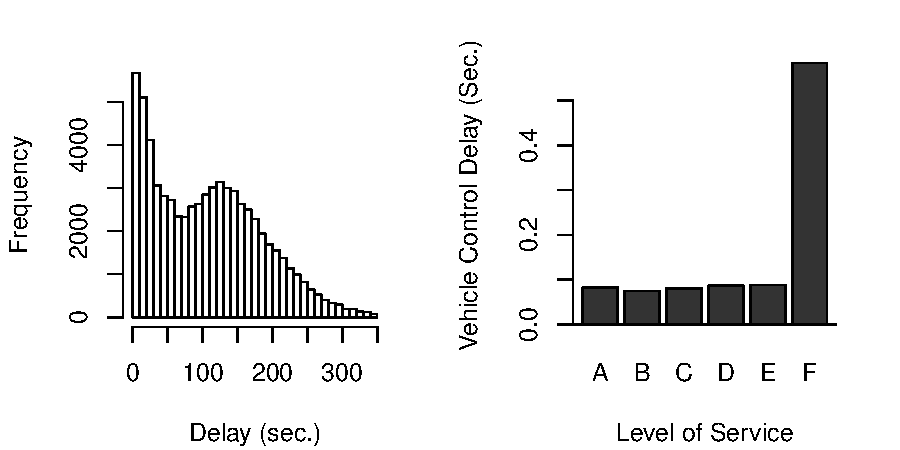
\includegraphics{upstat_report-LOCplot}
\caption{\leftskip0.25in\rightskip0.25in The Culver Road/East Main Street
intersection has a poor Level of Service. The histogram on the left shows the
distribution of the average vehicle control delay for each observation. The
distribution is bimodal with peaks at zero seconds and 140 seconds. The median
delay was 103 seconds with a IQR of
123 seconds. The bar plot on the right shows the
distribution of each LOS grade for each observation in our data set.
Observations were given a letter grade based on the average vehicle control
delay for each 5 minute interval. The majority of all observations had a delay
of greater than 80 seconds, suggesting that the intersection is predominantly grade
F.}
\label{fig:LOSfigure}
\end{figure}

We also examined the relationship between the traffic density and traffic volume,
also known as flux. Whe plotted, the relationship between the traffic density
and the traffic volume creates the fundamental diagram of traffic flow
\cite{HCM}, as shown in Figure \ref{fig:Fundamental}. Using linear regression techniques, we
were able to estimate the free flow velocity to be 19.5 miles per hour and the
traffic wave velocity to be 2.43 miles per hour against the direction of traffic.
We also determiend thecritical traffic density to be 42.8 vehicles per mile.
As the vehicle denisty passes the critical density, the traffic flow becomes
more unstable leading to traffic waves and congestion. To maximize
the traffic flow, the vehicle density must remain below the critical density.

\begin{figure}[h]
\centering
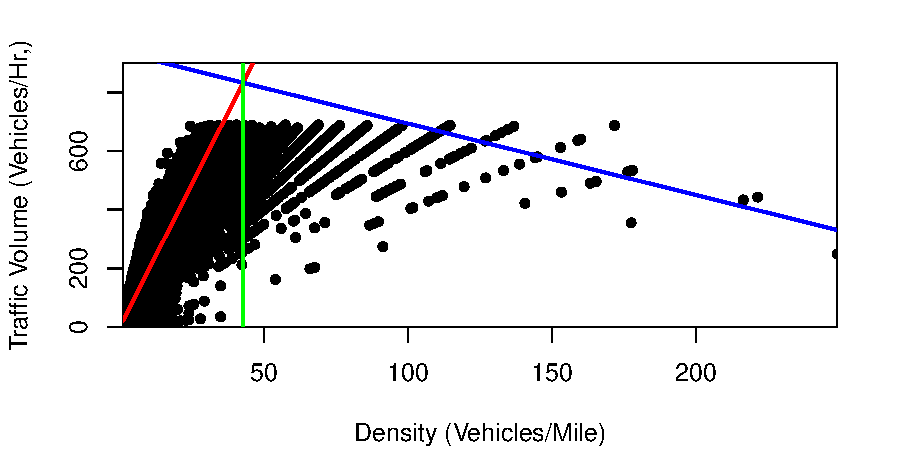
\includegraphics{upstat_report-003}
\caption{\leftskip0.25in\rightskip0.25inFundamental diagram of traffic flow provides
free flow and traffic wave velocities. Traffic density was calculated by
dividing the traffic volume by the traffic speed. Using linear regression, we
found the free flow velocity (19.5 mph) as depicted in red, the traffic wave
velocity (2.43 mph) as depicted in blue, and the critical density (42.8 vehicles
per mile) as depicted in green.}
\label{fig:Fundamental}
\end{figure}


\subsection*{Trend and Pattern Analysis}

To examine the general trend in the metrics we were provided, we performed linear
and multivariate regression. These techniques allows us to approximate the traffic
volume and delay. Figure \ref{trends} shows the median delay for each week and
the median traffic volume for each week with the linear regression for each data
set. Our data suggest that the median amount of time that vehicles wait at the
intersection may be increasing by 0.24 seconds per week. Our data also suggest
that the median number of vehicles utilizing the intersection may be increasing
by approximately 11 vehicles per week. Although the correlation coefficients are
rather low, we are confident that the traffic congestions will worsen as more
vehicles utilize the intersection.

\begin{figure}[H]
\centering

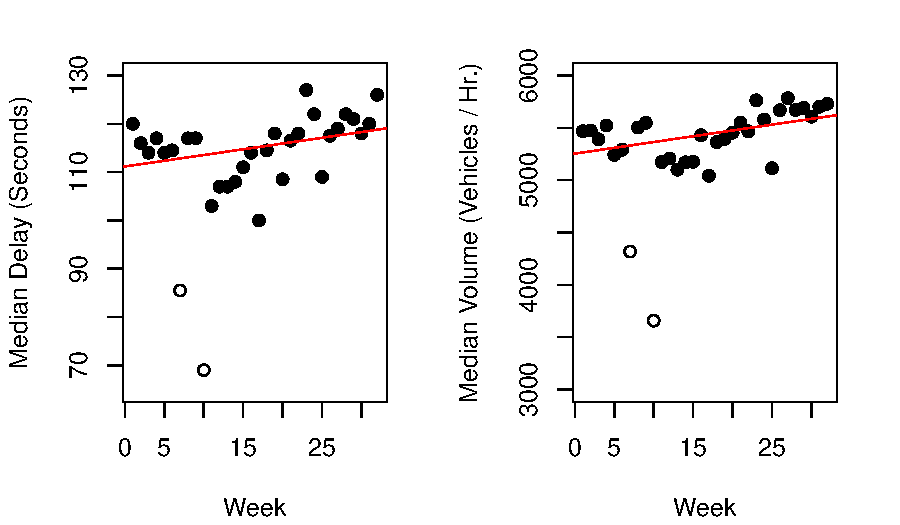
\includegraphics{upstat_report-VolumePlot}
\caption{\leftskip0.25in\rightskip0.25in The median traffic delay and median weekly
traffic volume are increasing over time. A linear regression of the median
traffic delay for each week suggests that the traffic delay may be increasing
0.24 seconds per week
($R^2 = 0.13$). Similarly, a linear
regression of the median number of vehicles to pass through the intersection per
week suggests that the number of vehicles utilizing the intersection may be
increasing at a rate of 11.08 vehicles
per week ($R^2 = 0.24$).}
\label{trends}
\end{figure}

We can also use the recorded vehicle volumes for each day to detect traffic
abnormailties as a means of locating interesting traffic patterns. To perform this
analysis we constructed template days of the week, seven traffic time series that
are the median traffic volume for every 5 minute interval. We then calculated the
correlation between the weekday template and the day of interest for each day in
our data set. A plot of each day's correlation, as shown in Figure \ref{fig:correlation},
outlines the variablity in each day's traffic patterns. An apt example of abnormal
driving is the seventh Thursday of the data set, which corresponds to Thanksgiving.
The 2013 Thanksgiving traffic was abnormally low for a Thursday. Similarly, the
10th and 20th Wednesdays of the data set exhibit similar patterns of minimal traffic..

\begin{figure}[h]
\centering
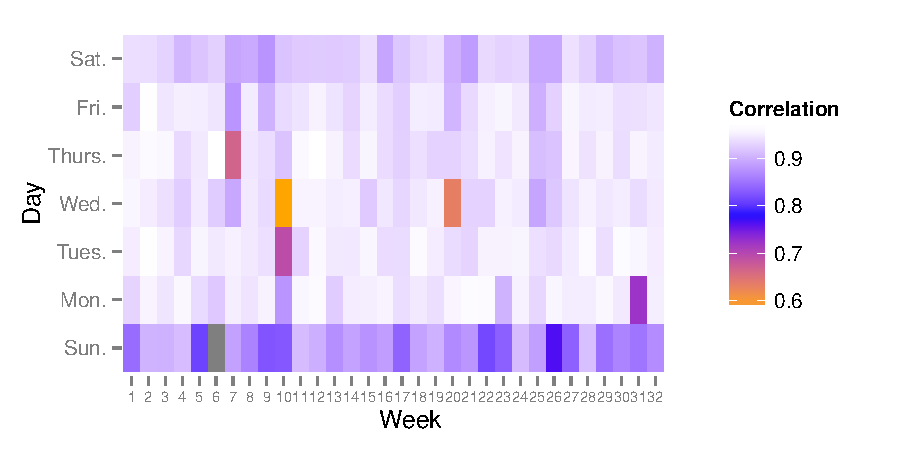
\includegraphics{upstat_report-006}
\caption{Correlation analysis shows holidays, data collection errors, and small-scale
traffic patterns. In this color scale, white indicates high correlation, purple
indicates moderate correlation, and orange indicates low correlation. Some days of
interest include the seventh Thursday, which corresponds with Thanksgiving, the
10th Tuesday and Wednesday, and the 20th Wednesday.}
\label{fig:correlation}
\end{figure}

We can directly compare the low traffic seen on the 10th Wednesday
(December 18, 2013), a typical Wednesday like October 16, 2013 and Thanksgiving.
As seen in Figure \label{fig:wednesday}, the traffic pattern exhibited by December
18, 2013 is very similar to that of Thanksgiving and not similar to a typical
Wednesday.

\begin{figure}[H]
\centering
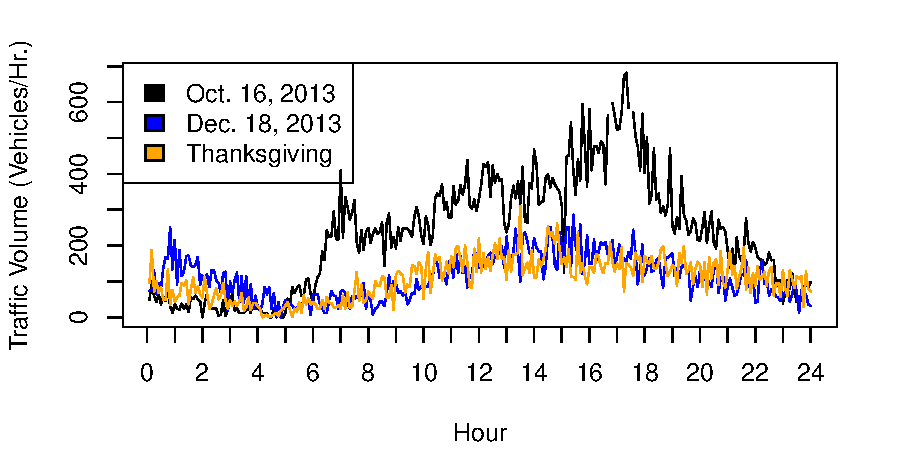
\includegraphics{upstat_report-007}
\caption{The traffic from December 18, 2013 is similar to Thanksgiving holiday traffic.}
\label{fig:wednesday}
\end{figure}

\subsection*{Bayesian Analysis}

\begin{figure}[H] \label{fig:bayesplot}
\centering
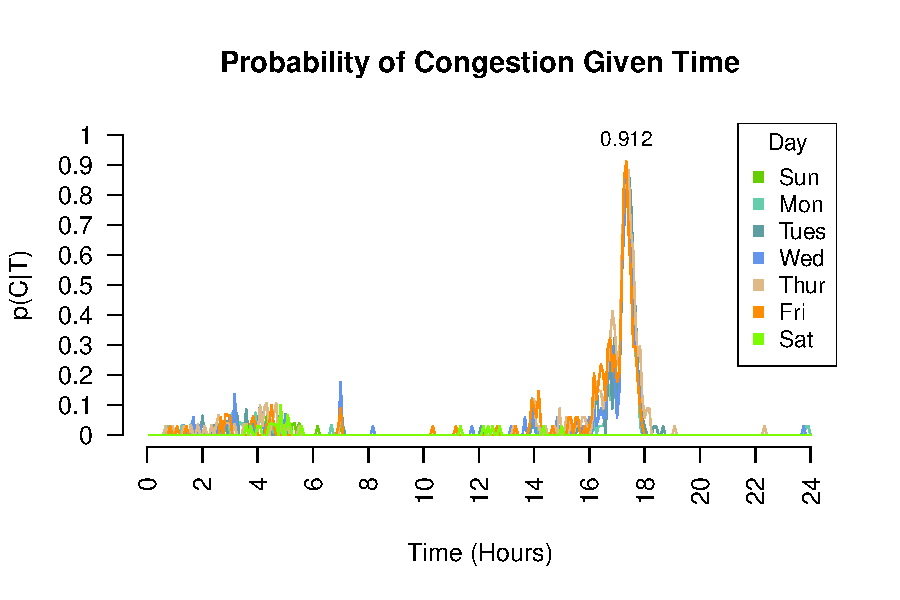
\includegraphics{upstat_report-bayesplot}
\caption{\leftskip0.25in\rightskip0.25in Probability of observing congestion based on specific times throughout the day (represented as p(C|T)). All days are represented as separate lines. A maximum probability of 91.2\% is shown on the graph and occurs at 5:15pm on Friday. Most weekdays have the highest probability of congestion between 5:00pm and 5:25pm, or during evening rush hour.}
\end{figure}

In order to determine how the probability of congestion relates to the time of day we adapted Bayes' Theorum for use with the data provided. Because the traffic on the weekend is not as intense as the traffic during the weekdays, the decision was made to evaluate each day independently of one another so as not to induce any sort of bias into the results. Congestion was determined simply by using the critical density of the intersection, identified as 42.8 Vehicles per Mile. Any situation where the density is equal to or greater than this measure is determined to be 'congested.' Any situation below this measure is simply 'not congested.'

This is then sorted for each time step, and a proportion is generated about how many times (on a specific day of the week) that particular time is considered congested. For example, this means that if 2 out of the 10 observations at 2:10am on Wednesdays is considered to be congested, equal or exceeding the critical density, the proportion is calculated to be 0.2. This is then multiplied by the probability of congestion at any time amongst all the observations, and is then divided by the probability of randomly selecting that time from the dataset. The results for each day are shown in \ref{fig:bayesplot}.

\begin{table}[h] \label{bayestable}
\centering
\caption{Selected results from Bayesian analysis of traffic data. These times represent the highest probability of observing traffic congestion. Saturday and Sunday were omitted from the table due to the fact that their relative probabilities were approximately zero.}
\begin{tabular}{l|l
>{\columncolor[HTML]{EFEFEF}}l l
>{\columncolor[HTML]{EFEFEF}}l l}
\textbf{Time} & \textbf{Mon} & \textbf{Tues}                & \textbf{Wed} & \textbf{Thur} & \textbf{Fri}                                         \\ \hline
17:05         & 0.500          & 0.471                        & 0.529        & 0.588         & \cellcolor[HTML]{FFFFFF}0.500                          \\
17:10         & 0.765        & 0.824                        & 0.677        & 0.824         & \cellcolor[HTML]{FFFFFF}{\color[HTML]{333333} 0.853} \\
17:15         & 0.824        & {\color[HTML]{333333} 0.853} & 0.882        & 0.824         & 0.912                                                \\
17:20         & 0.853        & 0.882                        & 0.765        & 0.882         & 0.677                                                \\
17:25         & 0.588        & 0.794                        & 0.647        & 0.677         & 0.529
\end{tabular}
\end{table}

Furthermore, each weekday has a particularly high probability of congestion between 5:00pm in the afternoon and 5:30pm. The results of the Bayesian analysis are shown in \ref{bayestable} for increased clarity. Interestingly enough, this is also when the road typically has the highest vehicular flow or volume. Because the area directly north of the intersection is mainly residential, it is hard to understand what is causing all of the volume and congestion.

We could speculate that it is being used to circumvent other possibly congested roadways, however we lack the ability to determine that because we do not have the data.

\subsection*{Weather Analysis}
Praesent iaculis pulvinar justo eu cursus. Mauris a ex eget sapien finibus commodo. Aenean et malesuada nunc. Nam iaculis porttitor faucibus. Etiam consequat rhoncus eros ut vehicula. Mauris vel ligula non nisl posuere aliquet. Mauris ac pulvinar metus, feugiat faucibus metus. Proin vel gravida tellus. Phasellus quis metus sollicitudin, volutpat massa nec, euismod risus. Nunc iaculis pellentesque purus non lobortis. Nam ac neque varius, auctor velit in, pretium elit. Ut facilisis, lacus nec mattis aliquet, nisi sapien vehicula massa, nec pharetra velit orci ac magna. Pellentesque vel velit ornare, aliquam turpis sed, egestas lacus. Aliquam dapibus commodo nulla, nec tincidunt eros lacinia ut. Maecenas mi tellus, cursus at neque vitae, consectetur tempus eros.

Aenean maximus metus metus, in varius lorem ultrices in. Nulla a tortor tempus, facilisis orci in, viverra augue. Maecenas viverra mattis velit, et volutpat elit finibus eu. Curabitur eu diam sed justo malesuada fringilla. Fusce ac nisl nec diam aliquam lobortis. Fusce fermentum ligula dui, vel condimentum erat convallis vitae. Etiam finibus dolor et feugiat iaculis. Duis varius nulla non dictum rutrum. Curabitur aliquet turpis id turpis fringilla, laoreet interdum mauris dictum. Praesent id pharetra tortor, ac laoreet urna. Sed porta lacus non sagittis condimentum.
\noindent\section*{Recommendations}
Praesent iaculis pulvinar justo eu cursus. Mauris a ex eget sapien finibus commodo. Aenean et malesuada nunc. Nam iaculis porttitor faucibus. Etiam consequat rhoncus eros ut vehicula. Mauris vel ligula non nisl posuere aliquet. Mauris ac pulvinar metus, feugiat faucibus metus. Proin vel gravida tellus. Phasellus quis metus sollicitudin, volutpat massa nec, euismod risus. Nunc iaculis pellentesque purus non lobortis. Nam ac neque varius, auctor velit in, pretium elit. Ut facilisis, lacus nec mattis aliquet, nisi sapien vehicula massa, nec pharetra velit orci ac magna. Pellentesque vel velit ornare, aliquam turpis sed, egestas lacus. Aliquam dapibus commodo nulla, nec tincidunt eros lacinia ut. Maecenas mi tellus, cursus at neque vitae, consectetur tempus eros.

Aenean maximus metus metus, in varius lorem ultrices in. Nulla a tortor tempus, facilisis orci in, viverra augue. Maecenas viverra mattis velit, et volutpat elit finibus eu. Curabitur eu diam sed justo malesuada fringilla. Fusce ac nisl nec diam aliquam lobortis. Fusce fermentum ligula dui, vel condimentum erat convallis vitae. Etiam finibus dolor et feugiat iaculis. Duis varius nulla non dictum rutrum. Curabitur aliquet turpis id turpis fringilla, laoreet interdum mauris dictum. Praesent id pharetra tortor, ac laoreet urna. Sed porta lacus non sagittis condimentum.
Nuke Rochester.

\noindent
\section*{Cited Literature}

\begin{thebibliography}{9}
  \bibitem{HCM}
    Transportation Research Board of the National Academies,
    \emph{Highway Capacity Manual 2010}.
    5th edition,
    2010.
\end{thebibliography}

\end{document}
